% !TeX root=../main.tex
\chapter{پیاده سازی رویکرد گراف مبنا جهت موقعیت‌یابی و کالیبراسیون به صورت همزمان برای ربات کابلی}

در فصل قبل رویکردی بر مبنای ساختار گراف برای انجام مسئله کالیبراسیون و موقعیت‌یابی ربات به صورت زمان واقعی ارائه شد. ویژگی‌هایی برای این رویکرد ارائه شد که حل این مسئله پیچیده و پرکاربرد رباتیکی را تسهیل کرده و باعث بهبود نتایج بهینه‌سازی شده است. در این فصل پیاده‌سازی کاملی از گراف‌های معرفی شده بر روی یک ربات خواهیم داشت. سعی بر آن بوده که ربات انتخاب شده برای این پیاده‌سازی از نظر سینماتیک و دینامیک دارای معادلاتی نسبتاً پیچیده باشد تا قدرت و سرعت این الگوریتم را مورد بررسی کافی قرار دهیم.


\section{انتخاب ربات مناسب جهت توسعه الگوریتم}

ربات نمونه انتخاب شده برای ارائه این فرمول‌بندی، یک ربات چهار کابلی فروتحریک آسان نصب می‌باشد. علت انتخاب این نوع ربات آسان نصب به عنوان موضوع مورد بررسی، قابلیت استفاده زیاد آنها در کارکردهای متنوع رباتیکی می‌باشد، به شرطی که هر بار پس از نصب در هر محیط دلخواه فرآیند کالیبراسیون بدون زمان‌بر و با کمترین زحمت انجام شود. فرمول‌بندی انجام شده برای این ربات به نحوی است که منجر به یک کالیبراسیون خودکار در کنار موقعیت‌یابی تنها با همان حسگرهایی که ربات برای موقعیت‌یابی تعبیه شده است، بدون زحمت اضافی برای کاربر انجام می‌شود. نتیجه این رویکرد علاوه بر افزایش دقت نهایی این فرآیندها، مفهومی حقیقی‌تر به آسان نصب بودن به این دسته از ربات‌های کابلی می‌بخشد.

آنچه تا کنون بیشتر مورد بررسی قرار گرفته حل مسئله کالیبراسیون برای ربات‌هایی است که کابل آنها به عنوان جسمی صلب در نظر گرفته می‌شود. این فرض اساسی حل مسئله را آسان‌تر می‌کند. در ادامه‌ی این فصل ما با استفاده از رویکرد بیان شده، کالیبراسیون و موقعیت‌یابی را برای یک ربات کابلی با فرض یاد شده انجام می‌دهیم و نتایج را مورد بررسی قرار می‌دهیم. علی‌رغم اینکه این فرض حل مسئله را تا نگاهی ساده‌تر می‌کند، زمانی که نسبت جرم پنجه ربات به جرم کابل‌ها زیاد شود، این فرض قابل قبول نخواهد بود. نشان خواهیم داد که با افزایش این میزان شکم‌دهی که معمولاً در ربات‌هایی با ابعاد بزرگتر دیده می‌شود، کالیبراسیون و موقعیت‌یابی با مشکل مواجه خواهد شد.

تاکنون تحقیقات زیادی بر روی مدل‌سازی کابل‌های شکم‌دار انجام شده است که نتایج ارائه شده برای این مدل‌سازی‌ها از دقت بالایی برخوردار بوده‌اند. ما نیز برای حل مشکل کالیبراسیون و موقعیت‌یابی خود نیاز به وارد کردن این قیدها به مسئله هستیم. پیچیدگی‌های زیاد این مدل‌ها باعث شده است که کارهای اخیر در این حوزه نسبت به حل مسئله با این معادلات، از شبکه‌های عمیق برای این مدل‌سازی‌ها استفاده کنند که خود دارای مشکلاتی بوده و از دقت و اطمینان کافی بهره‌مند نیستند. روشی که ما برای حل این مشکل ارائه خواهیم کرد، مقیدسازی همان مسئله حل شده برای کابل‌های صلب بوده است. در انتها باری دیگر با حل این مسئله خواهیم دید که تمام آنچه که به عنوان مزیت‌های این رویکرد بیان کرده‌ایم در حل مسئله نمود پیدا می‌کنند و با سرعت و قدرت بالایی مسئله کالیبراسیون و موقعیت‌یابی به صورت همزمان برای این نوع ربات‌ها، بدون فرض صلب بودن کابل‌ها، که حل آنها در روش‌های مرسوم کاری بس دشوار بوده است، را حل می‌کنند.

\section{توسعه گراف عامل برای یک ربات چهار کابلی با فرض کابل صلب}
در این بخش، انجام فرآیند کالیبراسیون و موقعیت‌یابی به صورت همزمان برای یک ربات کابلی با در نظر گرفتن فرض صلب بودن کابل‌ها با رویکرد گراف-مبنا انجام می‌شود. برای این فرآیند، ابتدا ربات چهار کابلی ARASCam معرفی می‌گردد. سپس فرضیاتی بر روی ساختار ربات ایجاد شده و با در نظر گرفتن این فرضیات، فرمول‌بندی جامعی برای ربات ارائه می‌شود. در نهایت، از این فرمول‌بندی برای پیاده‌سازی گراف عامل معرفی شده استفاده می‌شود و نتایج مورد بررسی قرار می‌گیرد. 

\subsection{معرفی ربات کابلی ARASCam}
ربات \lr{ARASCam} که در گروه تحقیقاتی رباتیک \lr{ARAS} توسعه یافته است، یک ربات معلق فروتحریک موازی با کابل‌های محرک و با شش درجه آزادی می‌باشد. شکل 
\ref{fig:arascam}
 نسخه اولیه این  ربات که برای یک فضای کاری نسبتا کوچک آزمایشگاهی طراحی شده است را نشان می دهد. همانطور که در تصویر مشاهده می شود، پنجه ربات که مجهز به یک دوبین تعبیه شده بر روی پردازنده 
\lr{Raspberry PI} 
می باشد، توسط چهار کابل در فضا معلق شده است. $\boldsymbol{B}$ بیانگر دستگاه مختصات پایه و همچنین $\boldsymbol{E}$ نشاه دهنده دستگاه مختصات پنجه ربات می باشد. $i$ امین کابل در نقطه ${}^B\!\boldsymbol{b}_i$ در مختصات پنجه به ربات و در نقطه ${}^E\!\boldsymbol{a}_i$ در مختصات پایه به پولی متناظر آن متصل می شود. ماتریس انتقال از دستگاه مختصات پایه به پنجه با 
$\boldsymbol{T}^{\boldsymbol{B}}_{\boldsymbol{E}}$
نشان داده شده است.

\begin{figure}[t]
	\centering
	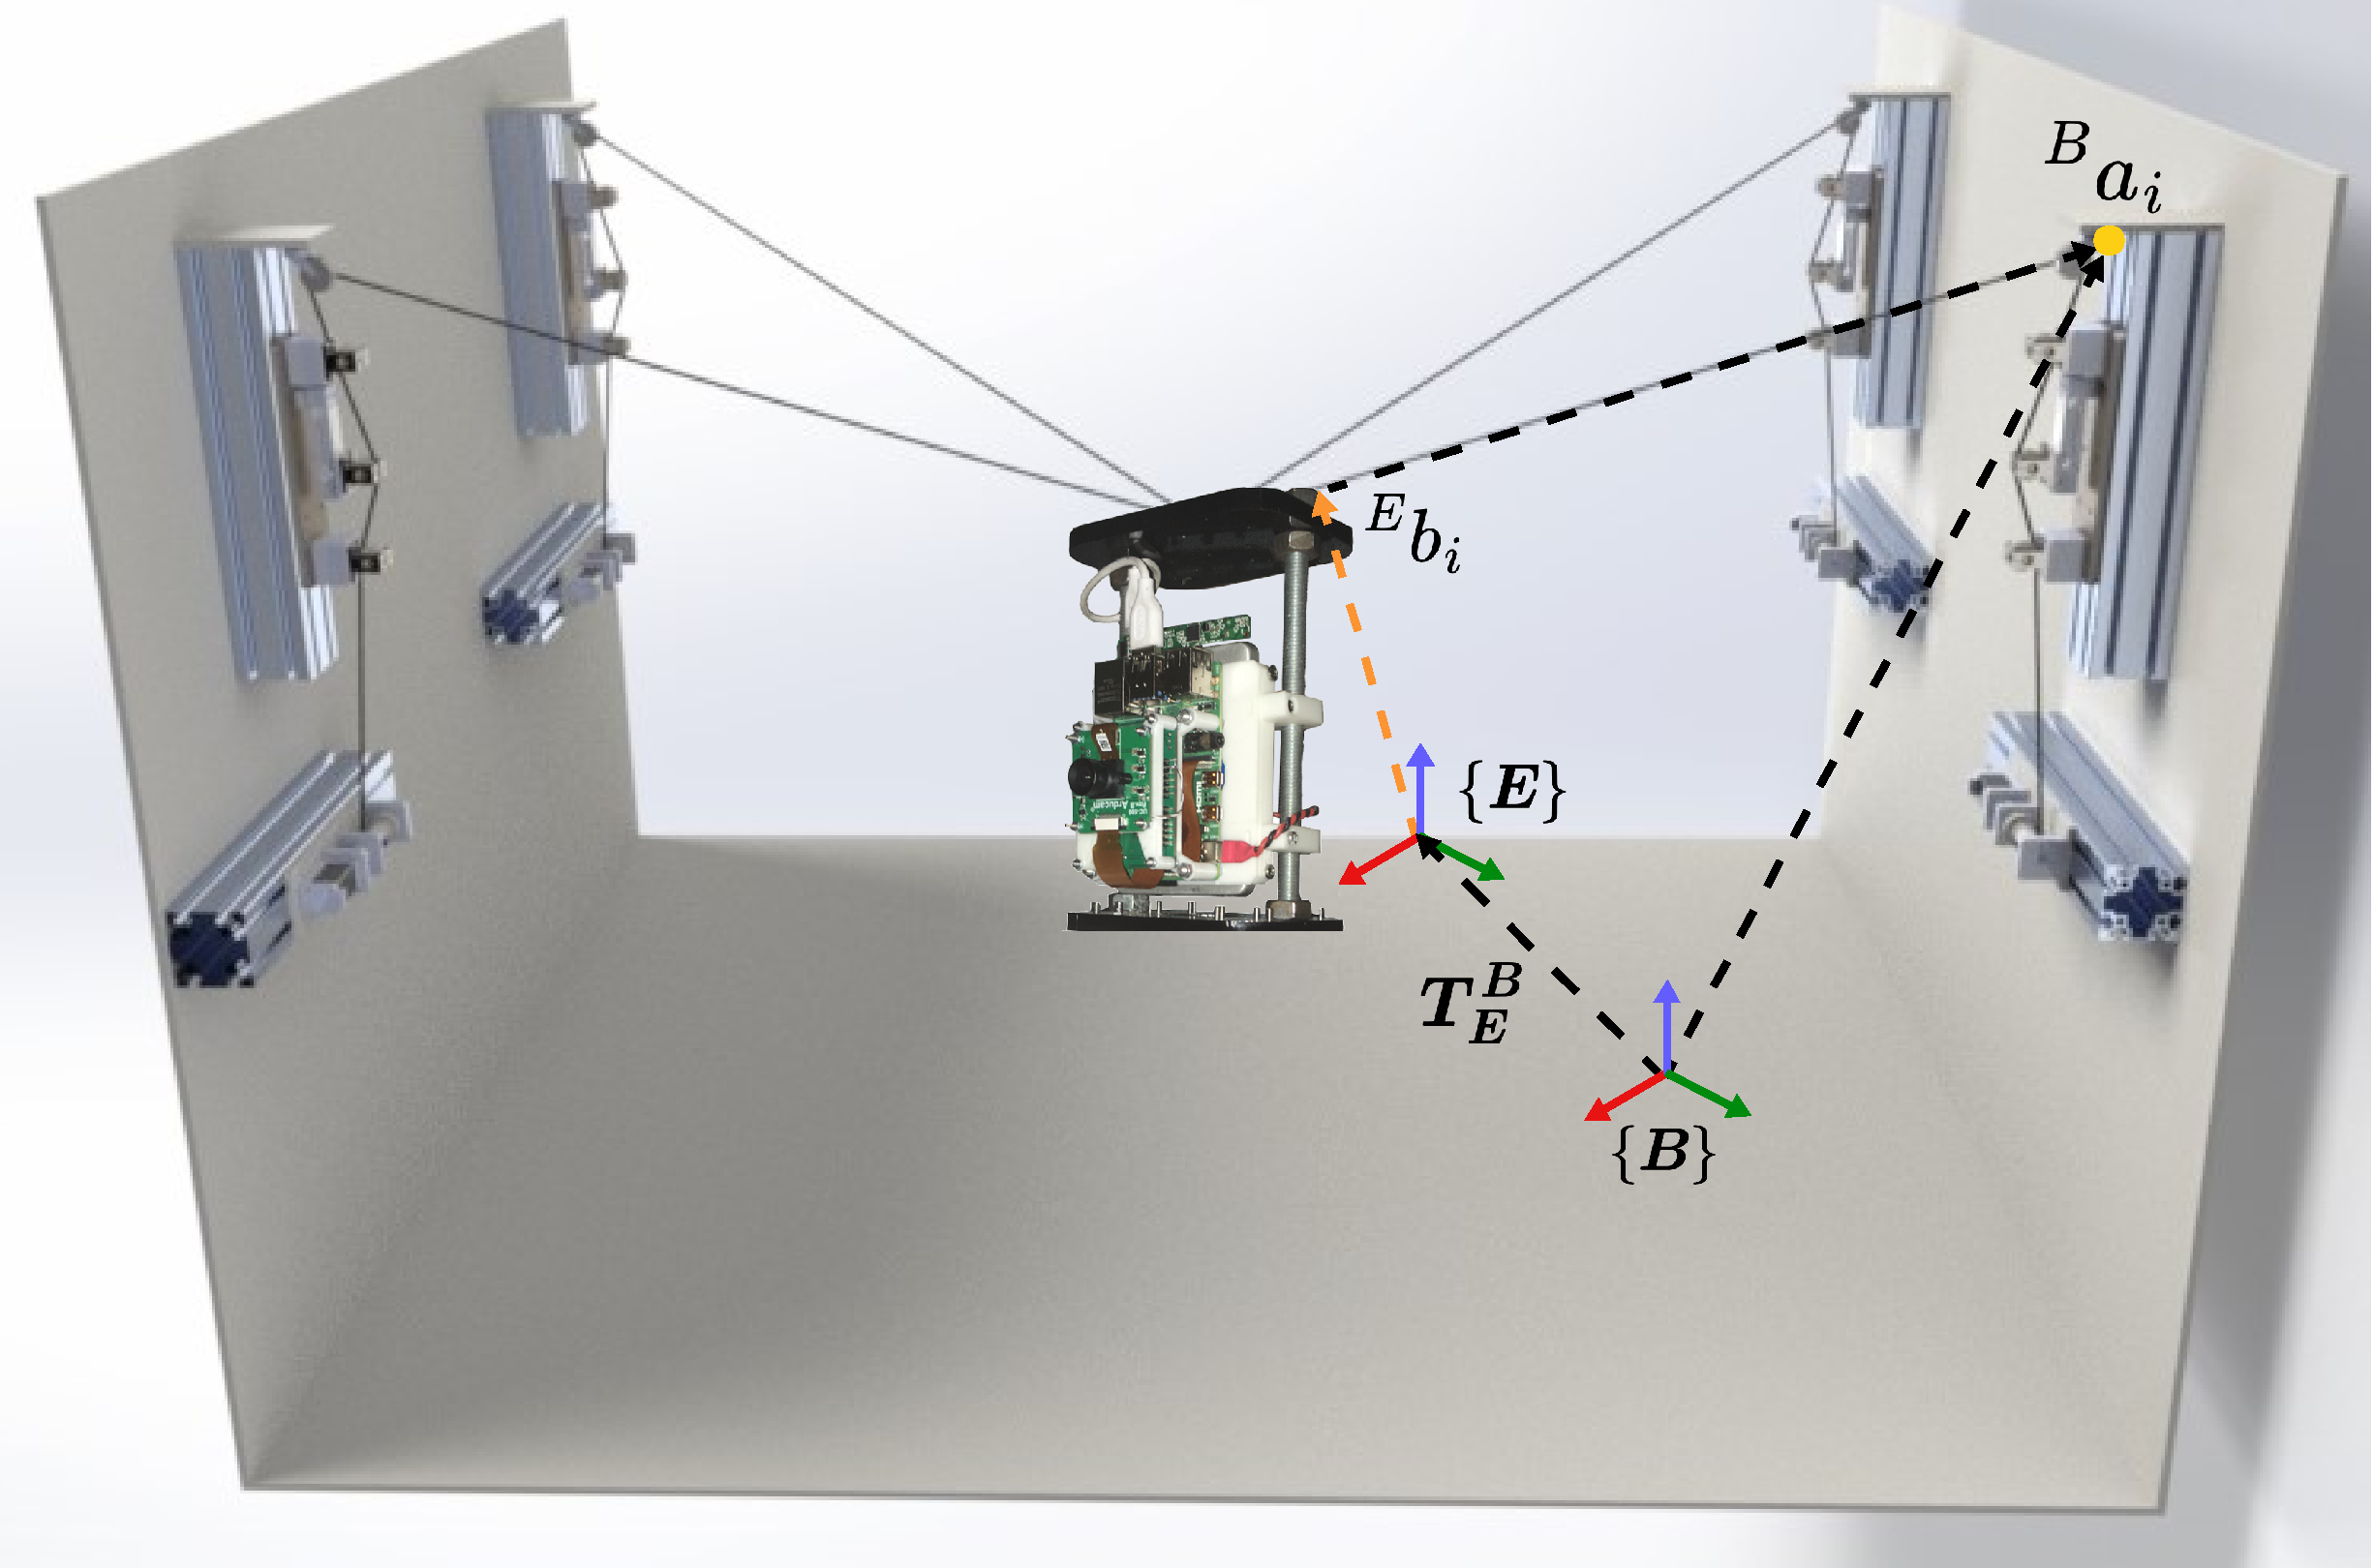
\includegraphics[width=0.7\linewidth]{img/arascam}
	\caption{}
	\label{fig:arascam}
\end{figure}

در این ربات، کابل‌ها با استفاده از یک سیستم مکانیکی درام جمع و باز می‌شوند. هر یک از کابل‌ها پس از خروج از درام، توسط مکانیزم مکانیکی از روی سنسور نیرو عبور کرده و سپس به پولی منتقل می‌شود. در نهایت، از نقطه مشخصی در پولی به ربات متصل می‌شود. همچنین از آنجایی که در این ربات نسبت جرم پنجه به جرم کابل‌های ربات مقدار زیادی است، می توان از شکم دهی کابل های آن صرف نظر کرد و کابل های آن را به عنوان اجسام صلب مدل کرد.

\subsection{بیان فرمول‌بندی مسئله و فرضیات}

برای فرمول‌بندی مسئله از هندسه بیان شده در شکل 
\ref{fig:arascam}
استفاده می کنیم. برای یک ربات با کابل‌های صلب، مدل اندازه‌گیری طول کابل \( \hat{z}_i \) با استفاده از حسگر انکودر روی ربات برای نمونه $k$، به صورت زیر می تواند فرمول‌بندی ‌شود:
\begin{equation}\label{eq:cable_length_without_young_module}
	\begin{split}
		l^\star_i [k] &\triangleq \| \boldsymbol{R}^B_E ~ {}^B\!\boldsymbol{b}_i + {}^B\!\boldsymbol{t}_E^B - {}^B\!\boldsymbol{a}_i \|^2 \\
		\hat{z}_i [k] &= l^\star_i [k] + l_{i}^0 + w_{\text{enc}} [k]
	\end{split}
\end{equation}


که در آن
\( (\boldsymbol{R}^B_E, {}^B\!\boldsymbol{t}_E^B) \)
 نشان‌دهنده ماتریس جهت‌گیری و بردار انتقال پنجه در دستگاه مختصات پایه،
\(l_{i}^0  \)
نشان‌دهنده مقدار جابجایی اولیه انکودر، و 
\( w_{\text{enc}} [k] \)
 نشان‌دهنده نویز اندازه‌گیری طول است. اگر انعطاف‌پذیری کابل نیز در نظر گرفته شود، نیروی
\( T_i \)
 در کابل، طول اندازه‌گیری شده کابل را به صورت زیر تغییر می‌دهد:
\begin{equation} \label{eq:cable_length_with_young_module}
	\hat{z}_i [k] = \left(1 - \frac{T_i [k] + w_T [k]}{EA} \right) l^\star_i [k] + l_{i}^0 + w_{\text{enc}} [k]
\end{equation}


که در آن \( E \) مدول یانگ کابل، \( A \) سطح مقطع کابل، و \( w_T [k] \) نویز اندازه‌گیری نیرو است. معادله 
\ref{eq:cable_length_with_young_module}
 بیان می‌کند که اگر نیروی کابل صفر باشد، \( T_i [k] = 0 \)، طول اندازه‌گیری شده توسط انکودر با فاصله واقعی بین \( a_i \) و \( b_i \) مطابقت دارد. با این حال، در پیکربندی‌ای که موتور در محل قفل شده و انکودر مقدار ثابتی را می‌خواند، جابجایی طول به دلیل کشیدگی توسط انکودر دیده نمی‌شود اما نسخه مقیاس‌شده وابسته به نیرو از فاصله واقعی \( l^\star_i [k] \) اندازه‌گیری می‌شود. با افزایش \( E \) (کابل‌های سفت)، اهمیت این مقیاس‌بندی وابسته به نیرو به صفر کاهش می‌یابد و معادله 
\ref{eq:cable_length_with_young_module}
به معادله
\ref{eq:cable_length_without_young_module}
 ساده می‌شود. در مورد ربات‌ با کابل‌های انعطاف‌پذیر، فرض می‌کنیم که حسگرهای نیروی کابل در نزدیکی عملگرها قرار گرفته‌اند. با این حال، برای بسیاری از کاربردها که به ربات‌های کابلی با اندازه متوسط نیاز دارند، انعطاف‌پذیری کابل ممکن است با انتخاب مناسب کابل‌ها قابل صرف نظر باشد.

علاوه بر فرمول‌بندی سینماتیک، مطابق شکل
\ref{fig:arascam}
 ربات با یک دوربین روی انتهای ربات، متصل به پنجه، تجهیز شده است. در اینجا ما تصاویر دریافتی از این دوربین را با استفاده از الگوریتم SVO برای تولید اندازه‌گیری‌های موقعیت ربات در فضای
$SE(3)$
به سیستم وارد می کنیم که بدین‌ترتیب موقعیت‌یابی ربات انجام شود:
\begin{equation}
	\Delta \boldsymbol{T}^k_{k-1} = \begin{bmatrix} R^k_{k-1} & t^k_{k-1} \\ 0 & s^{-1} \end{bmatrix}
\end{equation}

در طول مرحله کالیبراسیون و موقعیت‌یابی با استفاده از این الگوریتم، فرض می‌کنیم محیط‌ دارای نور خوب با بافت‌های غنی از ویژگی بوده و دوربین به آرامی حرکت می‌کند.  مسئله کالیبراسیون و مکان‌یابی به تخمین مشترک موقعیت‌های ربات
$\boldsymbol{T}^B_E [k]$,
موقعیت‌های نقاط اتصال کابل‌ها به پولی‌های متناظر
$\boldsymbol{a}_i$،
 طول‌های اولیه کابل‌ها
$l_{i}^0$،
و مقیاس الگوریتم مسافت‌پیمایی
$s$
با استفاده از اندازه‌گیری‌های الگوریتم مسافت‌پیمایی
 \( \Delta \boldsymbol{T}^k_{k-1} \)،
انکودرهای طول کابل
$z_i [k]$،
و برای ربات‌ها با کابل‌های انعطاف‌پذیر، اندازه‌گیری‌های نیرو 
$T_i$ 
کاهش می‌یابد.













این به حداقل‌رسانی عدم تطابق مدل-اندازه‌گیری سینماتیک به صورت زیر ترجمه می‌شود:

\[ \min_{a_i, l_{0i}, T^B_E [k], s} \sum_k \| h(a_i, l_{0i}, T^B_E [k], s) - z_i [k] \|^2_2 \]

که مدل اندازه‌گیری، \( h(.) \)، به صورت زیر تعریف می‌شود:

\[ h(a_i, l_{0i}, T^B_E [k], s) = s \left( 1 - \frac{\tau_i [k] + w_T [k]}{EA} \right) l^\star_i [k] + l_{0i} + w_{\text{enc}} [k] \]














%علی رغم اینکه در نظر گرفتن این فرض موجب کاهش یافتن بار محاسباتی و ساده تر شدن مسیله می شود، این فرض تا زمانی صادق خواهد بود که مطابق معیار ارایه شده در
%\cite{pott2013cable}
%نسبت جرم کابل به جرم مجری نهایی ربات قابل صرف نظر باشد. به عبارتی دیگر 